%File: formatting-instruction.tex
\documentclass[letterpaper]{article}
\usepackage{aaai}
\usepackage{times}
\usepackage{helvet}
\usepackage{courier}
\usepackage{amsmath}
\usepackage{color}
\usepackage{multirow}
\usepackage{diagbox}
\usepackage{graphicx}
\usepackage{makecell}
\usepackage{hyperref}
\usepackage{algorithm}
\usepackage{algpseudocode}
\hypersetup{hypertex=true,
colorlinks=true,
linkcolor=red,
anchorcolor=blue,
citecolor=blue}
\frenchspacing
\setlength{\pdfpagewidth}{8.5in}
\setlength{\pdfpageheight}{11in}
\pdfinfo{
/Title (AI Agents for Halma)
/Author (Put All Your Authors Here, Separated by Commas)}
\setcounter{secnumdepth}{0}  
 \begin{document}
% The file aaai.sty is the style file for AAAI Press 
% proceedings, working notes, and technical reports.
%
\title{AI Agents for Halma}
\author{Zhangzhi Xiong, Tianni Yang, Lingkang Feng\\
School of Information Science and Technology\\
ShanghaiTech University\\
{\tt\small \{xiongzhzh2023, yangtn2023, fenglk2022\}@shanghaitech.edu.cn}\\
}
\maketitle

\begin{abstract}
\begin{quote}


\end{quote}
\end{abstract}
% filepath: report/1-introduction.tex
\section{Introduction}
Halma is a strategy board game invented in the late 19th century, typically played on a checkered board by two players. The strategic depth of Halma, arising from its branching factor and long-term planning requirements, makes it an interesting testbed for artificial intelligence research. Figure~\ref{fig:halma} illustrates a typical Halma game setup in our code implementation.


\subsection{Rules}
In the original Halma rules, each player has multiple pawns and the objective is to transfer all of one's pieces from their starting corner or region to the diagonally opposite corner or region before the opponents do. Players take turns to move one pawn piece. Pieces can move to an adjacent square or jump over an adjacent piece (friendly or opponent) to the square immediately beyond it, with multiple jumps allowed in a single turn.
\begin{figure}[h]
    \centering
    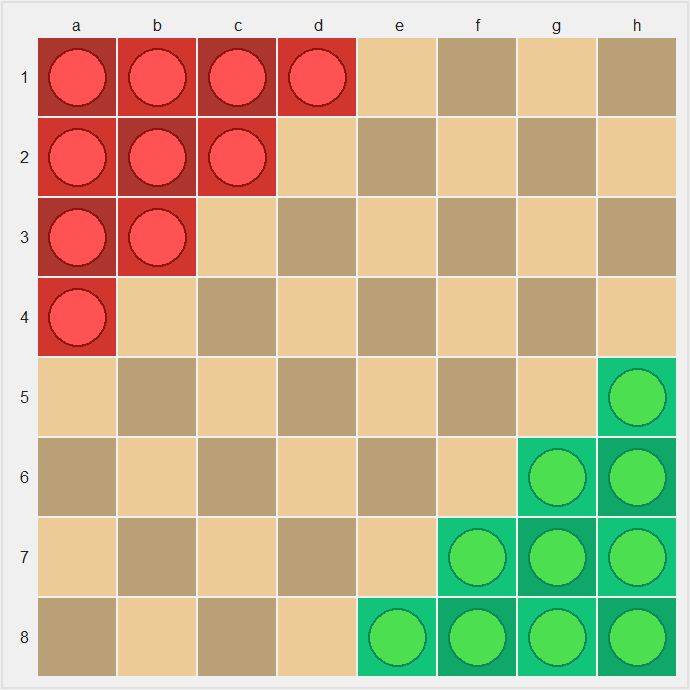
\includegraphics[width=1\columnwidth]{figures/halma.png}
    \caption{An example of a Halma game board and setup.}
    \label{fig:halma}
\end{figure}
\subsection{State Space}
In our game formulation, the board is 8$\times$8 and each player has 10 pawns. This means that the total number of state space is:
$$
\binom{64}{20} \times \binom{20}{10} = \frac{64!}{20! \cdot 44!} \times \frac{20!}{10! \cdot 10!} = \frac{64!}{44! \cdot 10! \cdot 10!} \approx 10^{28}
$$
\subsection{Motivation}

The motivation for this project is to use the knowledge about various agents in CS181 and deploy them in the scenario of Halma in practice. Also we seek to explore the impact of rules to our agents and see if there are any interesting findings when changing the rule a little bit. 

This report will introduce the design and implementation of several agents in CS181:
\begin{itemize}
    \item \textbf{Baseline agents:} \texttt{RandomPlayer} \item \textbf{Search agents:} \texttt{GreedyPlayer}
    \item \textbf{Adversary-Search agents:} \texttt{MinimaxPlayer} with alpha-beta pruning and optional local search heuristic.
    \item \textbf{Monte Carlo Tree Search:} \texttt{MCTSPlayer}\cite{DBLP:journals/corr/abs-2103-04931}
    \item \textbf{Reinforcement Learning agents:}
        \begin{itemize}
            \item \texttt{ApproximateQLearningPlayer}: Utilizes Q-learning with linear function approximation based on a rich set of handcrafted features and a tailored reward function.
            \item \texttt{Neural\_ApproximateQLearningPlayer}: Implements a Deep Q-Network (DQN)\cite{DBLP:journals/corr/MnihKSGAWR13} with a convolutional neural network\cite{DBLP:journals/corr/OSheaN15} for state representation, experience replay, and a target network.
        \end{itemize}
\end{itemize}

The competition results between these agents will be presented in this report. Moreover, we will discuss about how do we modify the rules and the corresponding interesting discoveries.

% filepath: report/2-method.tex
\section{Methodology}
In this section, we will introduce our implementation about our various agents based on the original rules.

\subsection{State Evaluation}
In search and adversarial search, state evaluation function is extremely important. It provides assessment information about a state and the agent will utilize  it and act accordingly.

In our implementation, our state evaluation function calculate the Euclidean distance from the pawn to every empty or non-player-occupied position in the player's goal area. If there are available goal positions, add the maximum of these distances to a running total.
If there are no available goal positions for that pawn, add 20 from the total as a penalty, since it indicates that there are opponents' remaining pawn in the area and moving towards the area may prevent them from leaving because of crowding pawns. 

After evaluating all pawns: Multiply the total score by -1, so that a smaller distance (i.e., pawns closer to the goal) results in a higher evaluation score. The state evaluation function equation is as follows:

\begin{equation}
\text{val} = - \sum_{p \in P_{\text{self}}} \left\{
\begin{array}{ll}
\max_{g \in G_{\text{empty}}} \text{dist}(p, g), & \text{if } G_{\text{empty}} \neq \emptyset \\
-20, & \text{if } G_{\text{empty}} = \emptyset
\end{array}
\right.
\end{equation}
where the distance is Euclidean one:
\begin{equation}
    \text{dist}(p, g) = \sqrt{(x_p - x_g)^2 + (y_p - y_g)^2}
\end{equation}

\subsection{RandomPlayer}
Every time \texttt{RandomPlayer} takes the turn, it will take a random valid action. 

\subsection{GreedyPlayer}
Every time \texttt{GreedyPlayer} takes the turn, it will take all the valid moves into account, and use the State Evaluation function to assess the corresponding following state as action score. Then \texttt{GreedyPlayer} will always choose the move with the maximum action score.

\subsection{Minimax Agent}
The \texttt{MinimaxPlayer} utilizes the classic Minimax algorithm, a recursive search enhanced with alpha-beta pruning and optional local search technique for efficiency.

\subsubsection{Core Algorithm}
\texttt{MinimaxPlayer} explores the game tree to a predefined depth due to rather large state space, assuming the opponent will always choose moves to minimize the Minimax player’s score. Alpha-beta pruning is employed to eliminate branches of the search tree that won't influence the final decision but significantly speeding up the search. In our experiments, Minimax agents has limited depth of two. 

\subsubsection{Local Search (Optional)}
If enabled, Local Search Heuristic aims to further prune the search space at each node of the Minimax tree and reduce the branching factor. Instead of considering all legal moves, it first evaluates the best possible move for each individual pawn based on the state evaluation score. Only this collection of best individual pawn moves is then considered by the Minimax algorithm. 


\subsection{Monte Carlo Tree Search Agent}
The \texttt{MCTSPlayer} utilizes Monte Carlo Tree Search\cite{DBLP:journals/corr/abs-2103-04931}, a probabilistic search algorithm that balances exploration of new possibilities with exploitation of known good paths.

\subsubsection{Core Process:} 
MCTS iteratively builds a search tree. Each iteration involves four phases as shown in Figure ~\ref{fig:mcts}:
\begin{figure}[h]
    \centering
    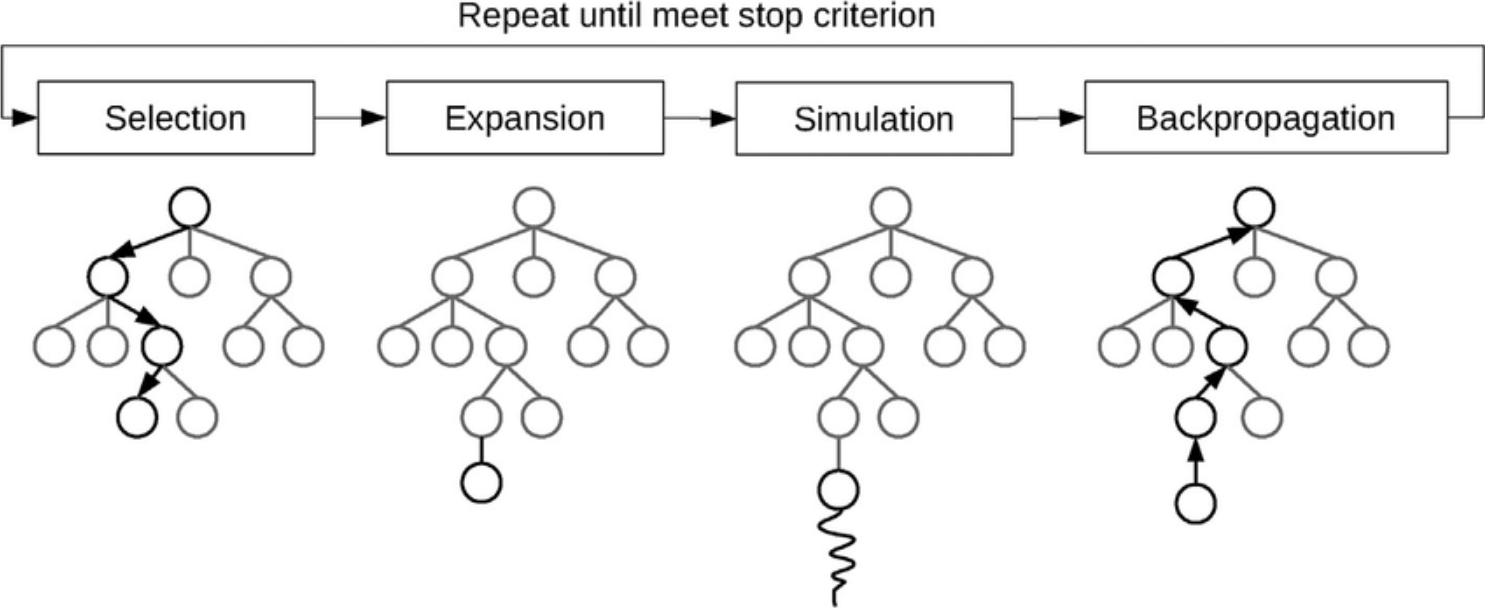
\includegraphics[width=1\columnwidth]{figures/mcts.png}
    \caption{Illustration of MCTS Core Process}
    \label{fig:mcts}
\end{figure}

\paragraph{Selection}
Starting from the root (current game state), the algorithm traverses the existing tree by repeatedly choosing child nodes that maximize the Upper Confidence Bound (UCB) criterion. In our implementation, the UCB formula is as follows:
\begin{equation}
    UCB = \frac{Q}{N} + c \sqrt{\frac{\ln N_{\text{parent}}}{N}} + \text{strategy\_score}
\end{equation}
where $Q$ is the cumulative value, $N$ is the visit count, $c$ is the exploration parameter and the $strategy\_score$ function for any move action $a$ is as follows:
\begin{equation}
StrategyScore(a) = 0.2 \times direction + jump
\end{equation}

\begin{equation}
direction=
\begin{cases} 
\frac{(x_e - x_s) + (y_e - y_s)}{2} & \text{if player } P_{\text{child}} \text{ is "RED"} \\
\frac{(x_s - x_e) + (y_s - y_e)}{2} & \text{if player } P_{\text{child}} \text{ is "GREEN"}
\end{cases}
\end{equation}

\begin{equation}
jump=
\begin{cases} 
0.3 & \text{if action } a \text{ is a jump} \\
0 & \text{otherwise}
\end{cases} 
\end{equation}
where $(x_e, y_e)$ stands for the position of the pawn after the move and $(x_s, y_s)$ stands for the one before the move. Note that in our implementation, Red Player's goal area is located at the right-bottom diagon and Green Player's goal area is located at the left-up diagon. The item \textit{direction} and \textit{jump} will encourage the agent to explore actions that move toward the goal area and jump, accordingly. 

\paragraph{Expansion}
If the selection process reaches a leaf node that is not a terminal game state and has untried actions, one new child node is added to the tree, corresponding to an untried action. Actions are prioritized for expansion based on heuristic scores (distance improvement, jump bonus, backward penalty).

\paragraph{Simulation}
From this new node (or a selected leaf if it's terminal), a simulated game (playout) is conducted. Actions during simulation are chosen using a fast, heuristic policy that favors moves improving distance to goal, direction, and jumps, with a small chance of random action selection. The playout continues until a game end-state or a depth limit.

\paragraph{Backpropagation}
The outcome of the simulation is propagated back up the tree from the expanded node to the root, updating the visit counts and value estimates of all traversed nodes. Under most circumstance, the simulation can't reach the end, hence requiring a \textit{Simulation Evaluation} function. We will soon introduce that. 

\subsubsection{Simulation Evaluation}
If a simulation ends due to depth limit rather than game completion, this function provides a heuristic score. In our implementation, we design a comprehensive simulation function heuristic which considers the number of pieces in the goal, the average distance of pieces to the goal, progressive bonuses for achieving stages of goal occupation, and penalties for pieces remaining in the starting area. The comprehensive monte carlo tree search simulation evaluation funciton is as follows for a state:
\begin{equation}
\begin{split}
Score_{\text{eval}} = \text{clamp}(Score_{\text{goal}} + Score_{\text{dist}} +
Bonus_{\text{stage}} + \\ Penalty_{\text{home}}, -1000, 1000)
\end{split}
\end{equation}
\begin{equation}
\text{clamp}(x, a, b) = \max(a, \min(x, b))
\end{equation}
\begin{equation}
Score_{\text{goal}} = 100 \times P_G
\end{equation}
\begin{equation}
Score_{\text{dist}} = 90 \times \left(1 - \frac{D_{\text{norm\_sum}}}{N_P}\right)
\end{equation}
\begin{equation}
Bonus_{\text{stage}} =
\begin{cases}
0 & \text{if } P_G = 0 \\
50 & \text{if } P_G = 1 \\
150 & \text{if } P_G = 2 \\
350 & \text{if } P_G = 3 \\
750 & \text{if } P_G \geq 4 
\end{cases}
\end{equation}
\begin{equation}
Penalty_{\text{home}} = -100 \times \frac{P_H}{N_P}
\end{equation}
where $P_G$ is the number of the player's pieces in the goal area,
$N_P$ is the total number of the player's pieces,
$D_{norm\_sum}$ is the sum of normalized Manhattan distances to the goal center for all pieces not in the goal, and 
$P_H$ is the number of the player's pieces in the home area and not moved. The intention of designing complicated simulation function is to provide a stronger evaluation with more inductive bias which may empirically contribute to the performance of our \texttt{MCTSPlayer}.

\subsubsection{Final Action Selection}
After a set number of simulations or a time limit, the agent chooses the action from the root's children that is most promising, based on a weighted combination of its win ratio, visit count, and a directional score.
\begin{equation}
\begin{split}
    score = 0.4 \times win\_ratio + 0.2 \times visit\_ratio \\ +  0.4 \times direction
\end{split}
\end{equation}

\begin{equation}
win\_ratio = \frac{child.value}{child.visits}
\end{equation}

\begin{equation}
visit\_ratio = \frac{child.visits}{root.visits}
\end{equation}

\begin{equation}
direction =
\begin{cases}
(x_e - start_x) + (y_e - y_s) & \text{if color is RED} \\
(x_s - x_e) + (y_s - y_e) & \text{otherwise}
\end{cases}
\end{equation}
where $(x_e, y_e)$ stands for the position of the pawn after the move and $(x_s, y_s)$ stands for the one before the move. This mechanism is to enhance our inductive bias and force \texttt{MCTSPlayer} to behave more wisely. Note that due to the complicated procedures, \texttt{MCTSPlayer} takes apparently more time in a turn to decide a move. 

\subsection{Q-learning Agent(Failed)}
Unfortunately, we failed to train a Q-learning agent. We tried letting Q-learning agent fight against random/minimax/Q-learning agents in limited episodes, but results in unintelligent behaviors. If setting the episodes larger, the q-state information file will be drastically large. This may caused by the rather large state space. According to our experiment, the file containing trained parameters after 200 episodes in .txt file is 21GB. When loading it into python, the program will crash.  

\subsection{Approximate Q-Learning Agent}
This agent learns to play Halma using Q-learning with linear function approximation. It utilizes various feature functions use linear combination with learnable weights to score a state. In short, the Q-value is approximated as a weighted sum of features: $Q(s,a) = \sum w_i f_i(s,a)$ where the weights $w_i$ can be learned.

\subsubsection{Feature Engineering}
In our implementation, we design a set of handcrafted features, $f_i(s,a)$, which describe the state-action pair. These include: normalized count of pieces in the goal, average distance of pieces to the goal, improvement in distance to goal due to the action, directional score of the action, and binary indicators for jumps, reaching the goal, moving backwards, or leaving the home area. Initial heuristic weights are assigned to these features.

In detail, our implemented feature functions and the final q-state approximation are as follows:
% State features
\begin{equation}
pieces\_in\_goal = \frac{\text{Number of player's pieces in goal area}}{4}
\end{equation}

\begin{equation}
avg\_distance = \frac{1}{4D_{\max}} \sum_{p \notin G} \left| x_p - x_c \right| + \left| y_p - y_c \right|
\end{equation}

% Action features
\begin{equation}
distance\_improvement = \frac{d_{\text{start}} - d_{\text{end}}}{D_{\max}}
\end{equation}

\begin{equation}
direction = 
\begin{cases} 
\frac{(x_{\text{e}} - x_{\text{s}}) + (y_{\text{e}} - y_{\text{s}})}{2B}, & \text{if RED} \\
\frac{(x_{\text{s}} - x_{\text{e}}) + (y_{\text{s}} - y_{\text{e}})}{2B}, & \text{otherwise}
\end{cases}
\end{equation}

\begin{equation}
is\_jump = 
\begin{cases} 
1, & \text{if jump move} \\
0, & \text{otherwise}
\end{cases}
\end{equation}

\begin{equation}
reaches\_goal = 
\begin{cases} 
1, & (x_{\text{e}}, y_{\text{e}}) \in G \\
0, & \text{otherwise}
\end{cases}
\end{equation}

% Additional action features
\begin{equation}
is\_backwards = 
\begin{cases} 
1, & \text{if move is backwards} \\
0, & \text{otherwise}
\end{cases}
\end{equation}

\begin{equation}
leaves\_home = 
\begin{cases} 
1, & (x_{\text{s}}, y_{\text{s}}) \in H \text{ and } (x_{\text{e}}, y_{\text{e}}) \notin H \\
0, & \text{otherwise}
\end{cases}
\end{equation}

\begin{equation}
\begin{split}
Q(s, a) = w_1 \cdot \text{pieces\_in\_goal} + w_2 \cdot  \text{avg\_distance} + 
\\ w_3 \cdot \text{distance\_improvement} + w_4 \cdot \text{direction} + \\ w_5 \cdot \text{is\_jump} + w_6 \cdot \text{reaches\_goal} + 
\\ w_7 \cdot \text{is\_backwards} + w_8 \cdot \text{leaves\_home}
\end{split}
\end{equation}

\subsection{Learning Mechanism}
Weights are updated using the Temporal Difference (TD) error. After taking an action $a$ from state $s$, observing reward $r$ and next state $s'$, the TD error is:
\begin{equation}
    \delta = r + \gamma \max_{a'} Q(s',a') - Q(s,a)
\end{equation}
Each weight $w_i$ is updated by:
\begin{equation}
w_i \leftarrow w_i + \alpha \cdot f_i(s,a)
\end{equation}
where $\alpha$ is the learning rate and $\gamma$ is the discount factor.

In our implementation, we support two approach for learning the weights: \textit{learning while fighting} and \textit{specific training}. For \textit{learning while fighting}, we use an empirically promising initial weights and use $\epsilon$-greedy strategy to update the weights and take actions during the competition. For \textit{specific training}, we have a specific training script of letting the agent to fight against minimax when being sente or gote, and update the weights.

According to our experiments and attempts, \textit{learning while fighting} strategy performs much better than \textit{specific training}. Hence we solely consider the approximate q-learning agent with \textit{learning while fighting}.

\subsection{$\epsilon$-greedy}
The agent balances exploration (trying new actions) and exploitation (choosing the best-known action). With probability $\epsilon$, it explores (choosing a non-backward random move if possible); otherwise, it exploits by selecting the action with the highest current Q-value. The exploration rate $\epsilon$ dynamically adjusts based on game progress and decays over time.
\subsection{Reward Function}
In approximate q-learning, designing reward is also important. The Q-value will be tuned towards the pattern of reward function. We provide a multi-stage and comprehensive reward function of a state and corresponding action for our agent as follows:
\begin{equation}
\begin{split}
& \text{reward} = \mathbf{1}_{\text{win}} \cdot \left(3000 + 500 \times 4 \times pieces\_in\_goal\right)
\\
&+ \mathbf{1}_{goal\_progress > 0} \cdot \left[300 \times 2^{current\_pieces}\right]
\\
&+ 
\begin{cases}
200 \times distance\_improvement, & \text{if } 4 \times pieces\_in\_goal \geq 2 \\
100 \times distance\_improvement, & \text{otherwise}
\end{cases}
\\
&- \mathbf{1}_{avg\_distance^{new} > avg\_distance^{old}} \cdot 300
\\
&+ 
\begin{cases}
0, & \text{if } is\_jump = 1 \text{ and } 4 \times pieces\_in\_goal \geq 3 \\
50, & \text{if } is\_jump = 1 \text{ and } 4 \times pieces\_in\_goal \geq 2 \\
200, & \text{if } is\_jump = 1 \text{ and } 4 \times pieces\_in\_goal < 2 \\
0, & \text{otherwise}
\end{cases}
\\
&-
\begin{cases}
500, & \text{if } is\_backwards = 1 \text{ and } 4 \times pieces\_in\_goal \geq 2 \\
200, & \text{if } is\_backwards = 1 \text{ and } 4 \times pieces\_in\_goal < 2 \\
0, & \text{otherwise}
\end{cases}
\end{split}
\end{equation}
In short, it provides large rewards for winning, scaled bonuses for pieces entering the goal, rewards for distance improvement (scaled by game stage), penalties for moving backward, and dynamic bonuses for jumps (larger in early game). The intention of designing complicated and comprehensive reward function is to make the reward more intuitively consistent with the real game reward pattern. 
% \end{itemize}

\subsection{Neural Approximate Q-Learning Agent (DQN)}
This agent implements a Deep Q-Network (DQN), a more advanced reinforcement learning technique that uses a neural network to approximate the Q-function. The unique components compared to Approximate Q-learning are Q-value network and DQN training paradigm. 
\subsection{Network Pipeline}
The pipeline of Network is as Figure ~\ref{fig:pipeline}. The input of network is Board state (4 channels) and action (4 dimensional). Board state has four channels encoding the board states containing player's pawns, opponent's pawns, player's goal area and opponent's goal area. The action is four dimensional since it has four data: $x_{\text{start}}, x_{\text{end}}, y_{\text{start}}, y_{\text{end}}$. The board vector will go through three convolutional layers (Conv2d)\cite{DBLP:journals/corr/OSheaN15} and action vector will go through a fully connected layer. These two processed vector will be concatenated and fed into three fully connected layers and eventually output Q-value. This is a regression model. 
\begin{figure}[h]
    \centering
    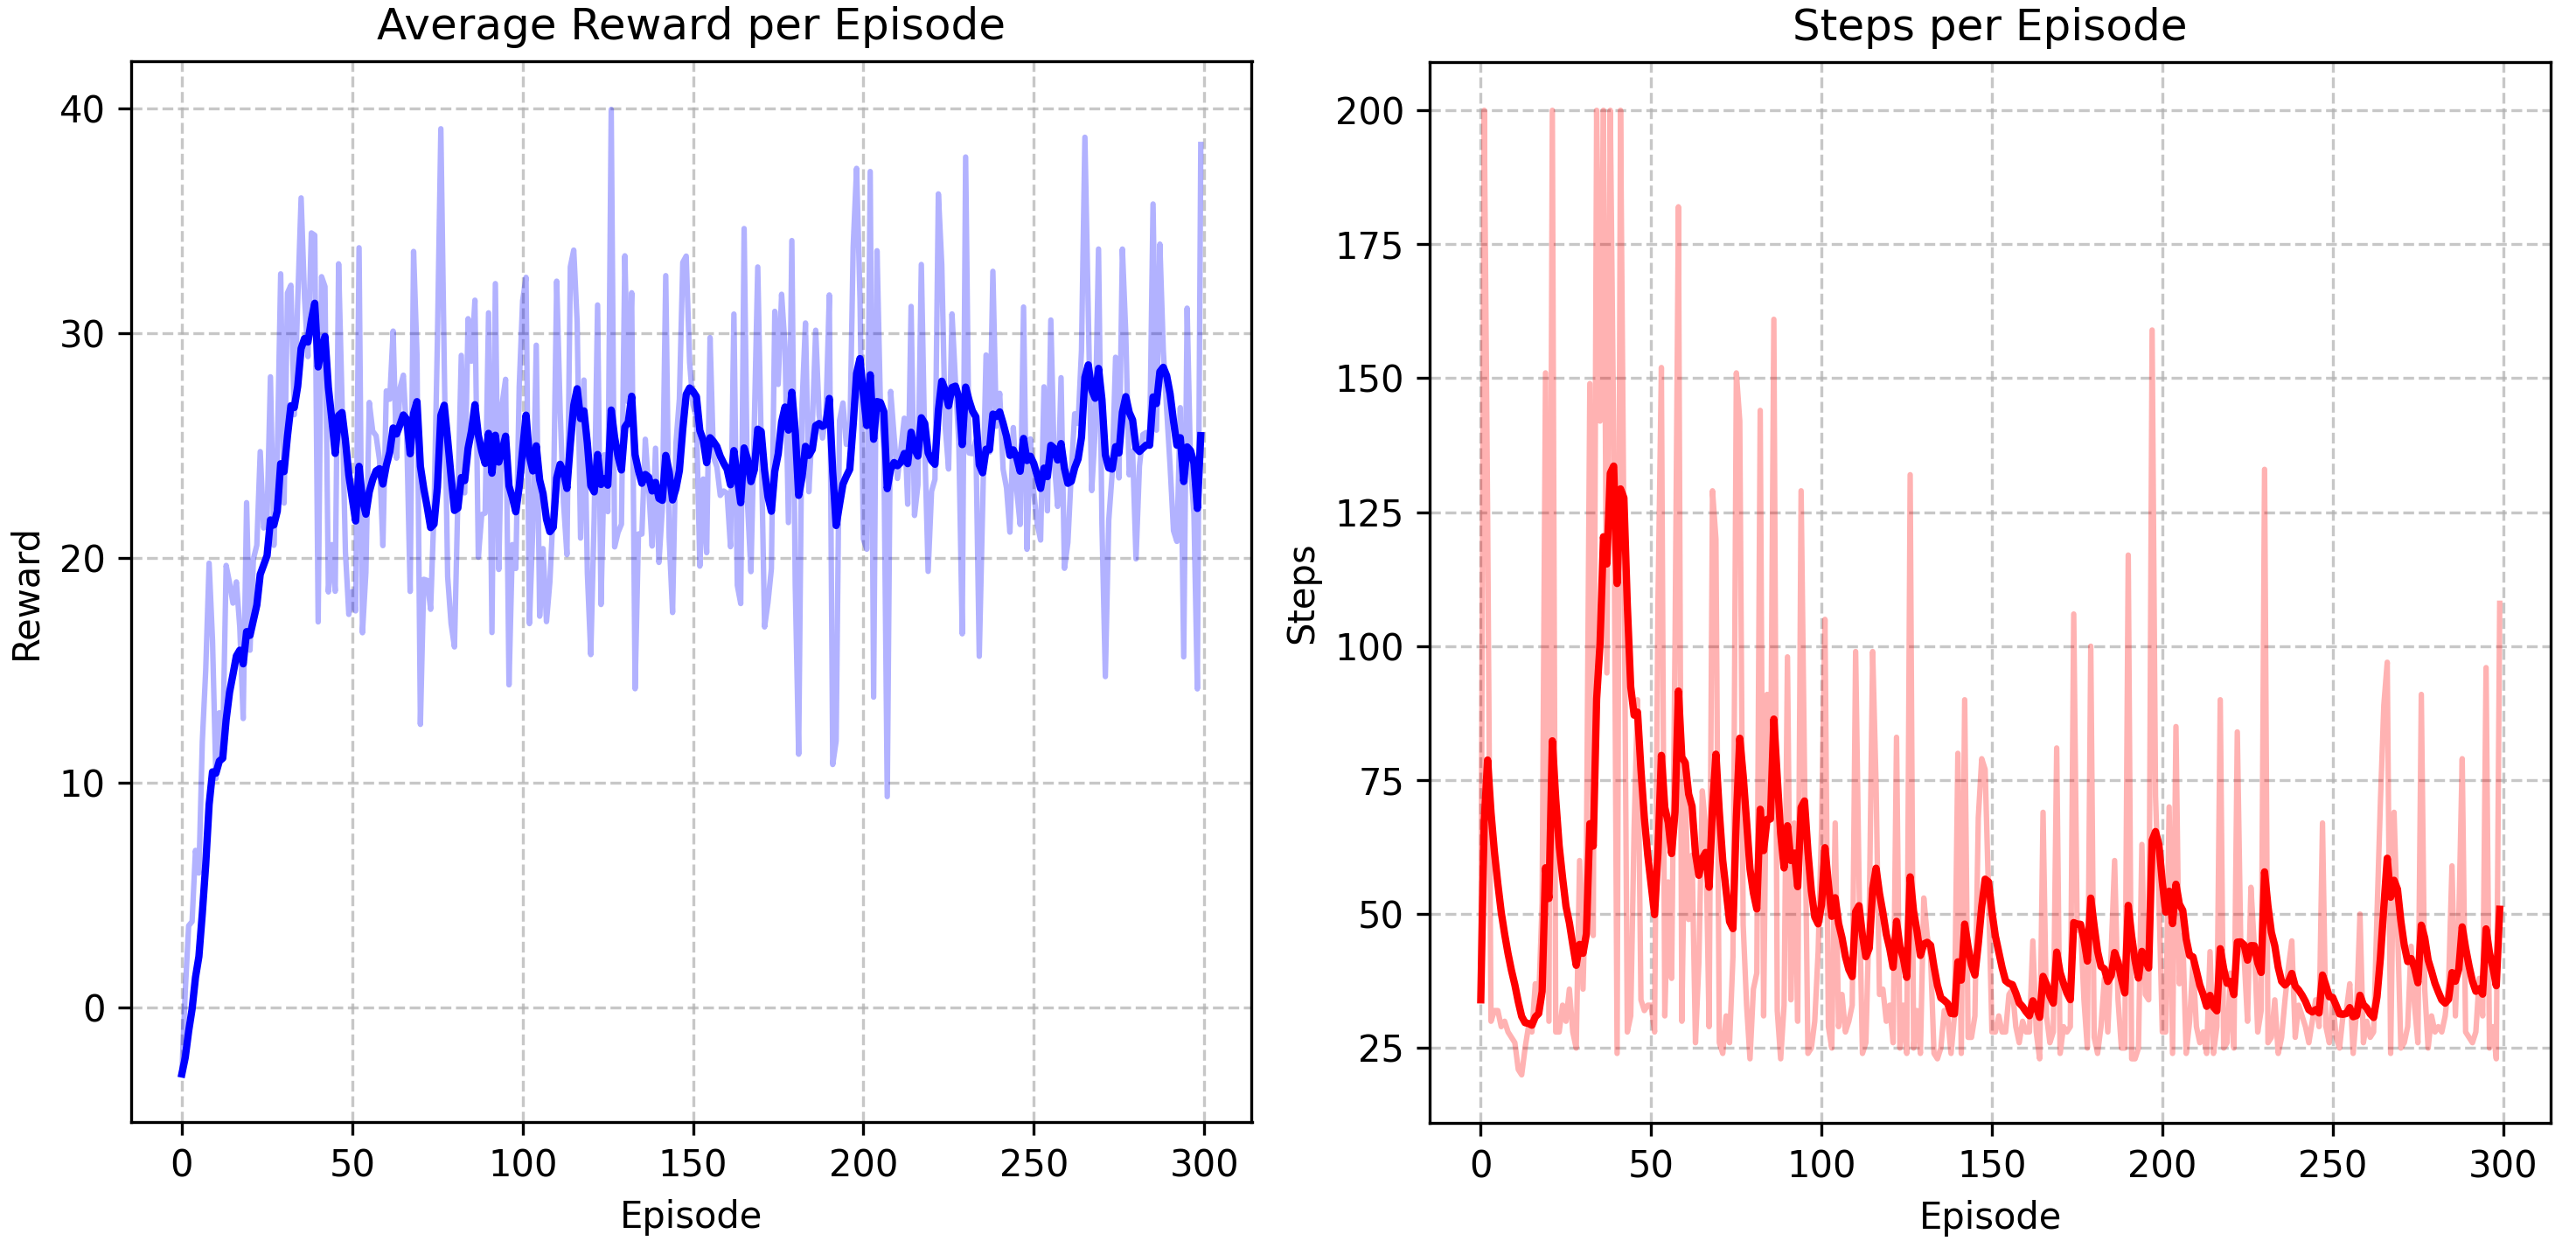
\includegraphics[width=1\columnwidth]{figures/sente.png}
    \caption{Training figure of sente side}
    \label{fig:sente}
\end{figure}
\begin{figure}[h]
    \centering
    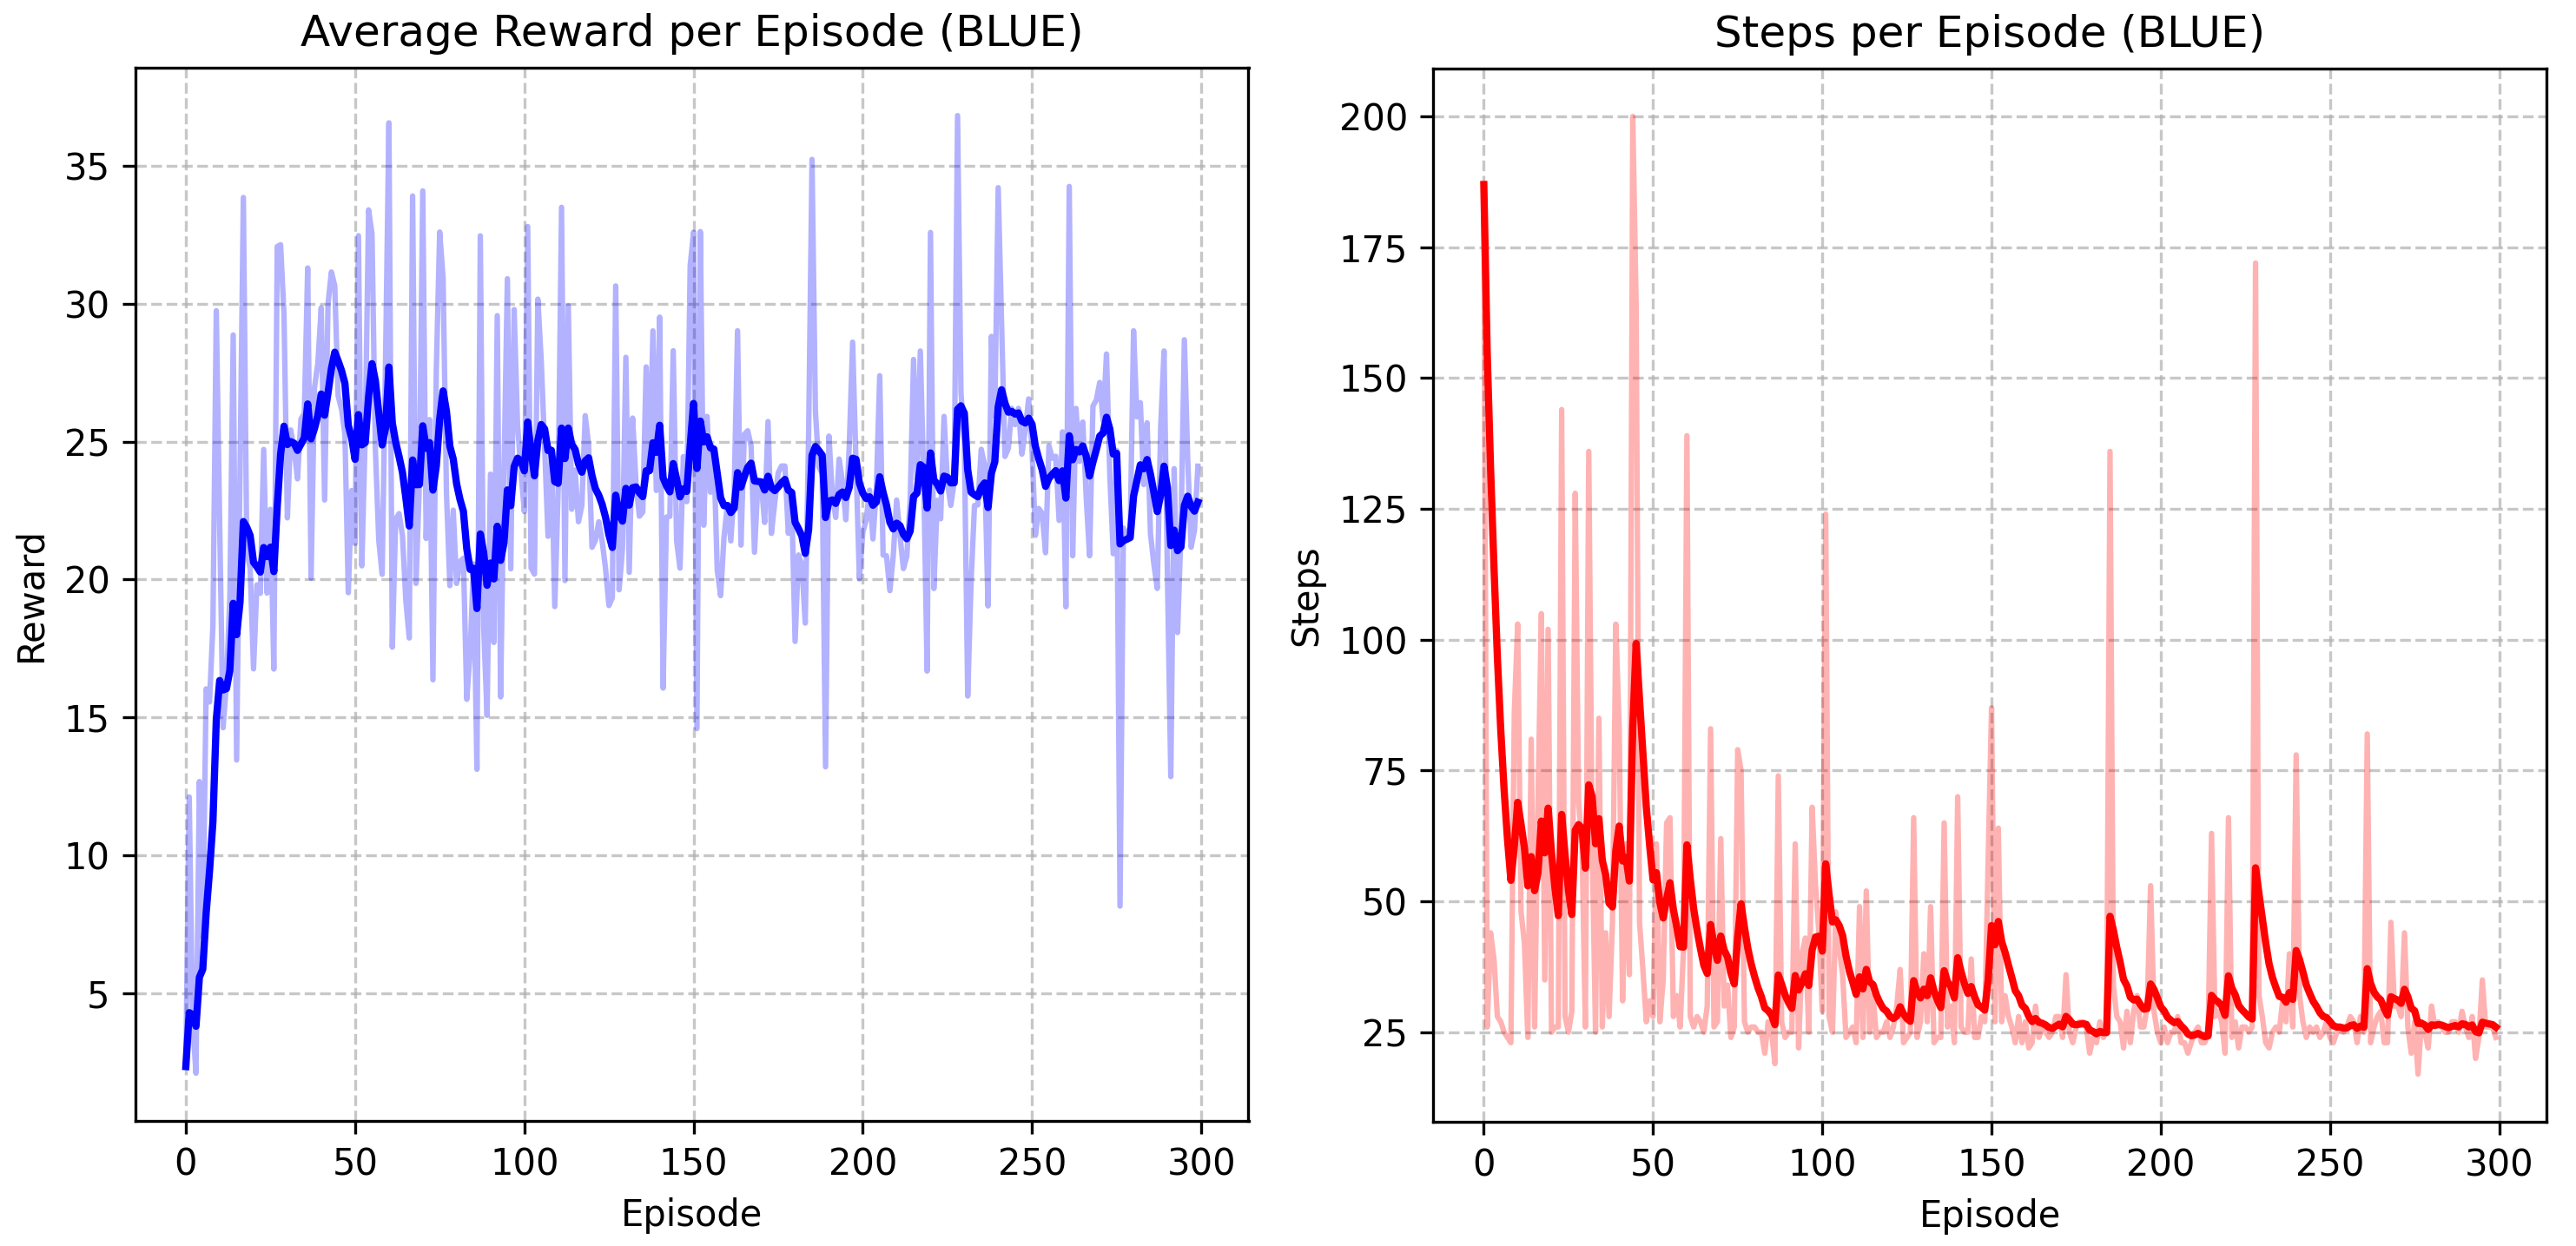
\includegraphics[width=1\columnwidth]{figures/gote.png}
    \caption{Training figure of gote side}
    \label{fig:gote}
\end{figure}
\begin{algorithm}[H]
\caption{Deep Q-learning with Experience Replay}
\label{alg:dqn}
\begin{algorithmic}[1]
\State Initialize replay memory $\mathcal{D}$ to capacity $N$
\State Initialize action-value function $Q$ with random weights
\For{episode $= 1, M$}
    \State Initialize sequence $s_1 = \{x_1\}$ and preprocessed sequenced $\phi_1 = \phi(s_1)$
    \For{$t = 1, T$}
        \State With probability $\epsilon$ select a random action $a_t$
        \State otherwise select $a_t = \max_{a} Q^*(\phi(s_t), a; \theta)$
        \State Execute action $a_t$ in emulator and observe reward $r_t$ and image $x_{t+1}$
        \State Set $s_{t+1} = s_t, a_t, x_{t+1}$ and preprocess $\phi_{t+1} = \phi(s_{t+1})$
        \State Store transition $(\phi_t, a_t, r_t, \phi_{t+1})$ in $\mathcal{D}$
        \State Sample random minibatch of transitions $(\phi_j, a_j, r_j, \phi_{j+1})$ from $\mathcal{D}$
        \State Set $temp = \gamma \max_{a'} Q(\phi_{j+1}, a'; \theta)$
        \State Set $y_j = \left\{
            \begin{array}{ll}
                r_j & \text{for terminal } \phi_{j+1} \\
                r_j + temp & \text{for non-terminal } \phi_{j+1}
            \end{array}
        \right.$
        \State Perform a gradient descent step on $(y_j - Q(\phi_j, a_j; \theta))^2$
    \EndFor
\EndFor
\end{algorithmic}
\end{algorithm}
\begin{figure}[h]
    \centering
    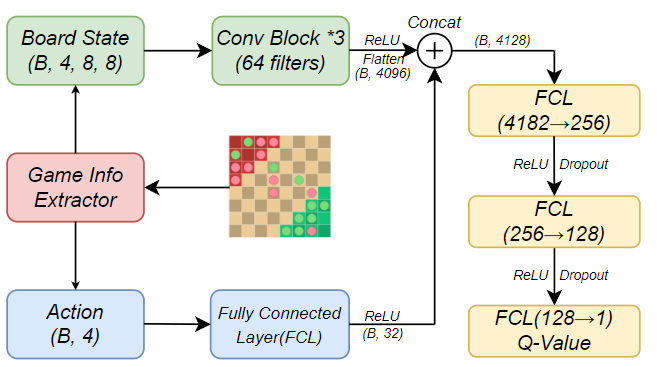
\includegraphics[width=1\columnwidth]{figures/pipeline.png}
    \caption{Pipeline of Network in DQN}
    \label{fig:pipeline}
\end{figure}
\subsection{DQN training paradigm}
The overall pseudocode about DQN\cite{DBLP:journals/corr/MnihKSGAWR13} training is presented in Pseudocode Algorithm ~\ref{alg:dqn}.

\subsubsection{Experience Replay}
Transitions (state, action, reward, next state, done flag) are stored in a replay memory. During training, mini-batches are randomly sampled from this memory to update the network. This breaks correlations between consecutive samples and improves learning stability.

\subsubsection{Target Network}
A separate "target" neural network, with the same architecture as the main Q-network, is used to generate the target Q-values for the TD error calculation ($R + \gamma \max_{a'} Q_{\text{target}}(s',a')$). The weights of the target network are periodically copied from the main Q-network, providing a more stable learning target.

\subsubsection{Learning Mechanism} 
The main Q-network is trained by minimizing the Mean Squared Error (MSE) between its predicted Q-values and the target Q-values computed using the target network and observed rewards. The Adam optimizer is used.
The related training figures in our experiments when training on the sente side and gote side are as Figure~\ref{fig:sente} and~\ref{fig:gote}.
\section{Results}

\section{External Resources}
We use Python to implement this project, using PyGame for GUI and game logic, Numpy for fast computation, and PyTorch for the Neural Network including convolution network, ResNet, and Linear network used in the improved Q-Learning. 
% filepath: report/4-rule.tex
\section{Rule Modification}
To encourage forward progress and strategic multi-jumping, we modified the rule and applied full experiments on it.

\subsection{Revised Experimental Setup}

We introduced two new parameters to encourage progress.
\begin{itemize}
  \item Maximum turns: 100.  
    If a match exceeds 100 turns, it ends in a draw to prevent score exploits through repetitive movements.
  \item Goal entry reward: 10 points per pawn entering the goal.
  \item Jump reward scalar (\texttt{jump\_scalar}):  
    For a sequence of \texttt{jump\_count} consecutive jumps, award \(\texttt{jump\_count} \times \texttt{jump\_scalar}\) additional points.
\end{itemize}

We first evaluate \(\texttt{jump\_scalar}\in\{1.0,1.2,1.5,2.0,5.0\}\), then conduct a binary search to find the value yielding roughly 50\% draws.

In Part (1) of the experiment, we evaluate agent performance under five different values of \texttt{jump\_scalar}: 1.0, 1.2, 1.5, 2.0, and 5.0. In Part (2), we apply a binary search strategy to determine the optimal value of \texttt{jump\_scalar} that results in approximately 50\% of the matches ending in a draw.

\subsection{Revised Winning Condition}

\begin{itemize}
  \item If all pawns enter goal areas within 100 turns, the higher-scoring player wins.
  \item Otherwise, the match is a draw.
\end{itemize}

\subsection{Revised Experiment Results}
Under the revised settings and winning conditions, we conducted head-to-head matches for Greedy, Minimax and Minimax Local Search players. Note that we limit our evaluation to G, M, and MLS, as other agent types are unable to fully exploit the additional rewards introduced by the revised rules. The outcomes of these matches are summarized and visualized using heatmaps to highlight win rates and performance differences across agents.

The revised results in part (1) are illustrated in the first five subplots in Figure~\ref{fig:jump}, where each cell indicates the win rate (in percentage) of the first player (Sente, row) when playing against the second player (Gote, column).

For clarity, the agents are abbreviated as follows: G (Greedy), M (Minimax), MLS (Minimax Local Search).

\begin{figure}[h]
    \centering
    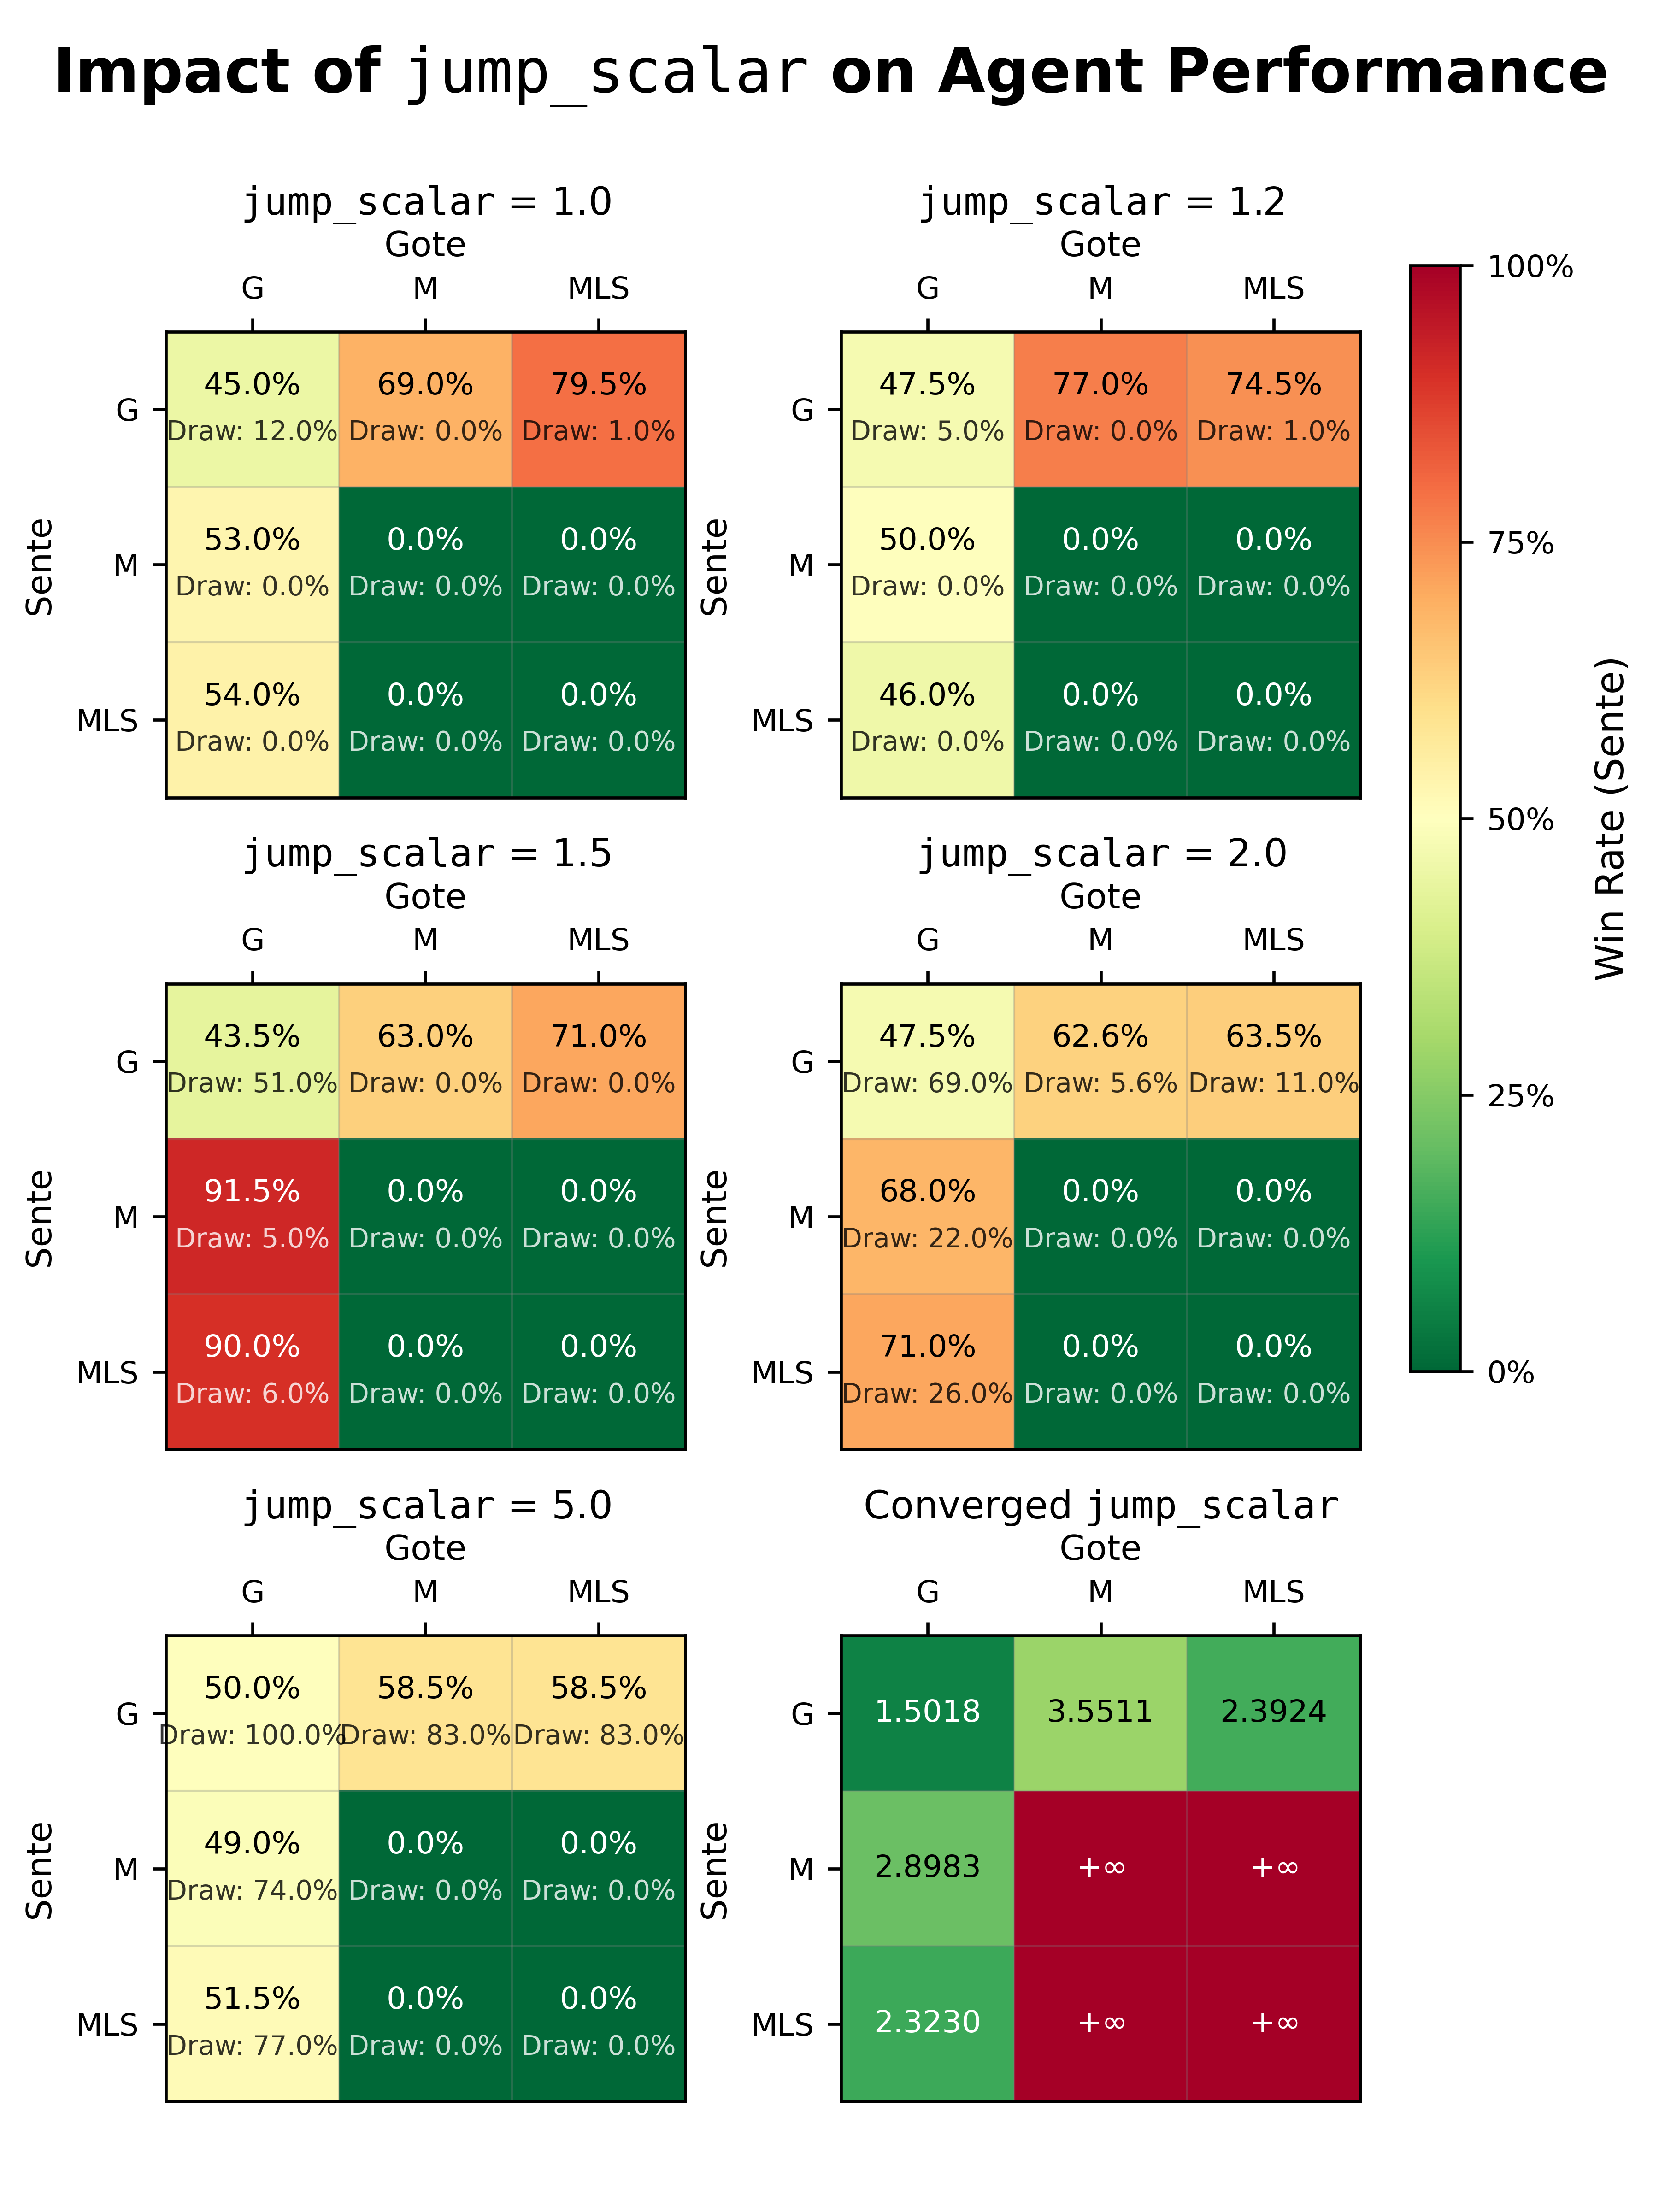
\includegraphics[width=1\columnwidth]{figures/jump_scalar.png}
    \caption{Impact of \texttt{jump\_scalar}}
    \label{fig:jump}
\end{figure}
% filepath: report/5-analysis.tex
\section{Analysis}

\subsection{Sente vs. Gote Advantage}
In Halma, the first player (Sente) and second player roles can influence outcomes due to the game's turn-based nature and board asymmetry. To assess this, we calculate the total wins for each agent across all matches.

Out of 2,990 games, Sente won 1,184 ($\approx 39.6\%$), and Gote won 1,806 ($\approx 60.4\%$), showing a substantial Gote advantage.

The two deterministic, depth-2 search agents (Minimax, MLS) are the main culprits—Sente never wins against itself, so every mirror match gives Gote a free +100\%. Stochastic or learning-based agents (Greedy, MCTS, AQL, NAQL) either swing the other way or stay close to parity, which is why the global numbers are not even more skewed.

\subsection{Strategy Performance Analysis}

\subsubsection{Greedy (G)}
The Greedy (G) agent, which selects uniformly at random from the set of actions that maximise a hand-crafted heuristic, achieves an impressive overall win-rate of roughly 80\%. Although it is conceptually simple and myopic, the stochastic tie-breaking injects a degree of variability that prevents opponents from over-fitting to a single deterministic line of play.

\subsubsection{Minimax (M)}
The Minimax (M) agent employs a two-ply $\alpha - \beta$ search with a static evaluation function. Owing to its fixed depth and the absence of any randomisation in move selection, its behaviour is fully deterministic. The shallow search horizon leaves it vulnerable to longer-term tactical refutations, which is reflected in its comparatively poor empirical performance.

\subsubsection{Minimax Local Search (MLS)}
The Minimax Local Search (MLS) agent augments the basic Minimax procedure with a local move-reordering heuristic that slightly improves the quality of its principal variations. While this modification yields a modest gain in win-rate relative to the plain Minimax player, the agent remains deterministic and inherits the same fundamental depth-limitation.

\subsubsection{Monte Carlo Tree Search (MCTS)}
The Monte Carlo Tree Search (MCTS) agent serves as a mid-level baseline. It balances exploration and exploitation through UCT and, by averaging over thousands of playouts, produces solid but unspectacular play. Empirically, its win-rate hovers around the centre of the field, outperforming the deterministic searchers yet falling short of the learning-based agents and the strong Greedy heuristic.

\subsubsection{Approximate Q‑Learning (AQL)}
The Approximate Q-Learning (AQL) agent represents each state–action value as a linear combination of domain-specific features updated via temporal-difference learning. Against search-based opponents—particularly the Minimax variants—it secures a clear statistical edge, indicating that even a relatively low-capacity function approximator can capture strategic patterns that elude shallow search.

\subsubsection{Neural Appraoximate Q‑Learning (NAQL)}
The Neural Approximate Q-Learning (NAQL) agent replaces the linear approximator with a deep neural network trained through self-play primarily against the Minimax family. This targeted curriculum yields dramatic gains: NAQL dominates both Minimax and MLS and remains competitive with Greedy and MCTS. Its performance underscores the advantages of high-capacity function approximation combined with adversarial training.

\subsection{Key Insights}
Collectively, the results demonstrate that no single paradigm is universally dominant. Simple, well-tuned heuristics (Greedy) can outperform more sophisticated search when the heuristic aligns closely with the game’s true value landscape. Conversely, shallow deterministic search (Minimax, MLS) is severely handicapped by its limited horizon, yet still provides useful sparring partners for reinforcement-learning agents. Stochastic, simulation-based methods (MCTS) achieve robust, “average-case” play but may lack the sharp tactical vision required to break strong heuristic lines. Finally, learning-based agents (AQL, NAQL) profit substantially from expressive value functions and targeted self-play, with NAQL’s neural representation delivering the largest leap in strength—particularly against the opponents it was trained to exploit.

\subsection{Impact of \texttt{jump\_scalar}}
To quantitatively analyse the effect of \texttt{jump\_scalar}, we evaluated five different parameter settings and observed that the proportion of draws rises sharply as \texttt{jump\_scalar} increases, while win-rate shifts are more nuanced.

For low multipliers ($\leq 1.2$) preserve the original “material advantage” meta-game. Greedy retains ~70–80\% win rates because quickly ferrying a pawn into the goal still outweighs speculative multi-hop routes.

For mid-range ($\approx 1.5$) is the tactical “sweet spot”. Search-based agents can finally monetise deeper look-ahead, toppling Greedy without letting games stagnate. Decisive results remain common (draw-rate only $\approx$ 10\%), so rankings are statistically meaningful.

For high multipliers ($\geq 2$) trade decisiveness for fairness. As hop chains dominate the reward landscape, missing one key sequence rarely leaves enough turns to recover; thus draws surge and inter-agent gaps narrow.

For very high multipliers (5) all but eliminate decisive outcomes, making the system useless for discrimination or learning feedback. Both of the players are more willing to jump repeatedly instead of jumping into goal area.

In summary, the analysis confirms that carefully tuned—but not extreme—jump incentives improve both efficiency and competitive performance, validating the heuristic design choice and providing a principled default value for downstream experiments.
% filepath: report/6-external.tex
\section{External Resource}
In this project, the GUI and framework are based on \url{https://github.com/indrafnugroho/halma}. We modify the code engineering to support using multiple agents conveniently and \texttt{classic} \& \texttt{score} two modes. 

Figure~\ref{fig:halma} is a screenshot of the game GUI in our project. Figure~\ref{fig:mcts} is borrowed from \href{https://paperswithcode.com/method/monte-carlo-tree-search} {\texttt{Paperwithcode}}. Pseudocode~\ref{alg:dqn} is borrowed and slightly modified from the pseudocode in the original DQN paper\cite{DBLP:journals/corr/MnihKSGAWR13}

The training for Neural Approximate Q-Leaning agent support \texttt{torch} and \texttt{CUDA}. The Figure~\ref{fig:sente}~\ref{fig:gote}~\ref{fig:heatmap}~\ref{fig:jump} are plotted with \texttt{Matplotlib}.
\newpage
\bibliography{ref} % Use the name of your .bib file without the .bib extension
\bibliographystyle{aaai} % Ensure this is present
\end{document}